\documentclass[a4paper,11pt]{article}
\usepackage[margin=22mm,headheight=15pt,headsep=8mm,footskip=11mm]{geometry}
\usepackage{amsmath,amssymb,booktabs,enumitem,fancyhdr,xcolor,tikz}
\usepackage[unicode,hidelinks]{hyperref}
\hypersetup{pdftitle={Stochastic Signal Analysis - Homework 2 Solutions}}
\pagestyle{fancy}\fancyhf{}
\fancyhead[L]{\small Stochastic Signal Analysis}\fancyhead[R]{\small Homework \#2: Solutions}
\fancyfoot[L]{\scriptsize Companion to the English exercise sheet}\fancyfoot[R]{\small\thepage\ / 10}
\setlength{\parindent}{0pt}\setlength{\parskip}{0.5em}\linespread{1.12}
\newcommand{\E}{\mathbb E}\newcommand{\Var}{\operatorname{Var}}\newcommand{\Cov}{\operatorname{Cov}}
\newcommand{\jj}{\mathrm j}\newcommand{\ee}{\mathrm e}
\newcommand{\problem}[3]{{\LARGE\bfseries Exercise #1}\hfill #2\par{\small\color{gray}Textbook p. #3}\par\vspace{3mm}}
\newcommand{\step}[1]{\par\textbf{#1}\par}
\begin{document}
\problem{2.3}{Required}{61}
One coin toss selects the entire sample function. At the two specified times,
\[
(X(1/2),X(1))=\begin{cases}(0,-1),&\text{heads, probability }1/2,\\(1,2),&\text{tails, probability }1/2.\end{cases}
\]
\step{(1) One-dimensional distribution functions}
Using the right-continuous convention $F(x)=P(X\le x)$,
\[
\boxed{F_X(x,1/2)=\begin{cases}0,&x<0,\\1/2,&0\le x<1,\\1,&x\ge1,\end{cases}}
\quad
\boxed{F_X(x,1)=\begin{cases}0,&x<-1,\\1/2,&-1\le x<2,\\1,&x\ge2.\end{cases}}
\]
\step{(2) Two-dimensional distribution function}
An atom contributes only when both of its coordinates meet the thresholds:
\[
\boxed{F_X(x_1,x_2;1/2,1)=\tfrac12\mathbf1_{\{x_1\ge0,\ x_2\ge-1\}}
+\tfrac12\mathbf1_{\{x_1\ge1,\ x_2\ge2\}}.}
\]
The two samples are not independent: they are determined by the same toss.
\step{(3) Graphs}
\begin{center}
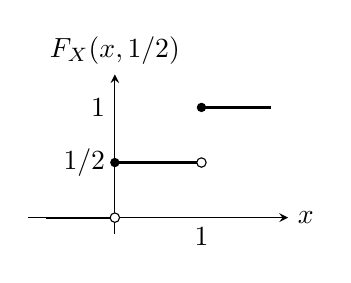
\begin{tikzpicture}[x=1.1cm,y=1.4cm,>=stealth]
\draw[->](-1,0)--(2,0)node[right]{$x$};\draw[->](0,-.15)--(0,1.3)node[above]{$F_X(x,1/2)$};
\draw[thick](-.8,0)--(0,0);\draw[thick](0,.5)--(1,.5);\draw[thick](1,1)--(1.8,1);
\foreach \x/\a/\b in {0/0/.5,1/.5/1}{\draw[fill=white](\x,\a)circle(1.7pt);\fill(\x,\b)circle(1.7pt);}
\node[below]at(1,0){$1$};\node[left]at(0,.5){$1/2$};\node[left]at(0,1){$1$};
\end{tikzpicture}\hspace{13mm}
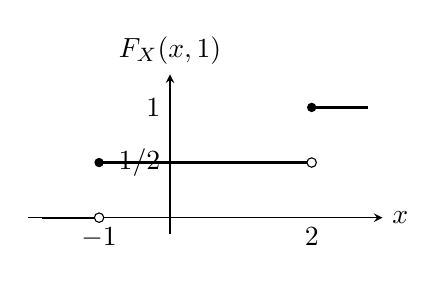
\begin{tikzpicture}[x=.9cm,y=1.4cm,>=stealth]
\draw[->](-2,0)--(3,0)node[right]{$x$};\draw[->](0,-.15)--(0,1.3)node[above]{$F_X(x,1)$};
\draw[thick](-1.8,0)--(-1,0);\draw[thick](-1,.5)--(2,.5);\draw[thick](2,1)--(2.8,1);
\foreach \x/\a/\b in {-1/0/.5,2/.5/1}{\draw[fill=white](\x,\a)circle(1.7pt);\fill(\x,\b)circle(1.7pt);\node[below]at(\x,0){$\x$};}
\node[left]at(0,.5){$1/2$};\node[left]at(0,1){$1$};
\end{tikzpicture}
\end{center}
The joint CDF is the following step surface, shown as a level map. Each region is a horizontal plateau at the labelled height; threshold lines belong to the region on their right or above.
\begin{center}
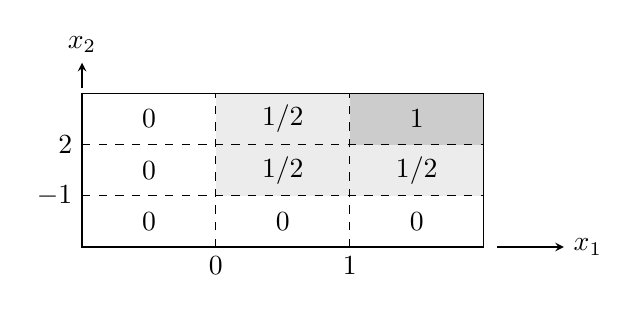
\begin{tikzpicture}[x=1.7cm,y=.65cm,>=stealth]
\fill[gray!15](1,1)rectangle(3,3);\fill[gray!40](2,2)rectangle(3,3);
\draw(0,0)rectangle(3,3);\draw[dashed](1,0)--(1,3);\draw[dashed](2,0)--(2,3);\draw[dashed](0,1)--(3,1);\draw[dashed](0,2)--(3,2);
\foreach \x/\y/\z in {.5/.5/0,1.5/.5/0,2.5/.5/0,.5/1.5/0,1.5/1.5/{1/2},2.5/1.5/{1/2},.5/2.5/0,1.5/2.5/{1/2},2.5/2.5/1}{\node at(\x,\y){$\z$};}
\node[below]at(1,0){$0$};\node[below]at(2,0){$1$};\node[left]at(0,1){$-1$};\node[left]at(0,2){$2$};
\draw[->](3.1,0)--(3.6,0)node[right]{$x_1$};\draw[->](0,3.1)--(0,3.6)node[above]{$x_2$};
\end{tikzpicture}
\end{center}
Outer regions extend to infinity. In the marginal graphs, filled endpoints are included.
\newpage
\problem{2.13}{Required}{62}
Let the resistance be $R>0$ and the capacitance be $C$. Both branches of a parallel RC circuit have the applied voltage $X(t)=A\cos(\omega t+\Theta)$.
\step{Total current}
With the passive sign convention, the resistor and capacitor currents are
\[
I_R(t)=\frac{X(t)}R,\qquad I_C(t)=C\frac{dX(t)}{dt}.
\]
For a given sample, $A$ and $\Theta$ are fixed with respect to time. Hence
\[
\frac{dX(t)}{dt}=-A\omega\sin(\omega t+\Theta),
\]
and Kirchhoff's current law gives
\[
\boxed{I(t)=A\left[\frac1R\cos(\omega t+\Theta)-\omega C\sin(\omega t+\Theta)\right].}
\]
\step{Mean-square value}
Write $\psi=\omega t+\Theta$. Since $A$ and $\Theta$ are independent,
\begin{align*}
\E[I^2(t)]
=\E[A^2]\bigl[&R^{-2}\E(\cos^2\psi)+\omega^2C^2\E(\sin^2\psi)\\
&-2\omega C R^{-1}\E(\sin\psi\cos\psi)\bigr].
\end{align*}
The amplitude is uniform on $[-1,1]$, so
\[
\E[A^2]=\frac12\int_{-1}^1a^2\,da=\frac13.
\]
Averaging over one complete phase period gives
\[
\E(\cos^2\psi)=\E(\sin^2\psi)=\frac12,\qquad
\E(\sin\psi\cos\psi)=0.
\]
For example, $\E(\cos^2\psi)=\frac1{2\pi}\int_{-\pi}^{\pi}\cos^2(\omega t+\theta)\,d\theta=1/2$.
Therefore the mean-square current is constant in time:
\[
\boxed{\E[I^2(t)]=\frac16\left(\frac1{R^2}+\omega^2C^2\right).}
\]
\newpage
\problem{2.16}{Required}{62}
\step{Mean, covariance, and Gaussianity}
Every finite collection of samples is a linear transformation of the jointly Gaussian vector $(A,B)$; therefore $X(t)$ is a Gaussian process. Independence and zero means give $\E[AB]=0$. Thus
\[
\E[X(t)]=0,\qquad
C_X(s,t)=\sigma^2[\cos\omega s\cos\omega t+\sin\omega s\sin\omega t]
=\sigma^2\cos\omega(s-t).
\]
In particular, $\Var[X(t)]=C_X(t,t)=\sigma^2$.
\step{One-dimensional density}
For $\sigma^2>0$, $X(t)\sim N(0,\sigma^2)$, so
\[
\boxed{f_X(x;t)=\frac1{\sqrt{2\pi}\sigma}\exp\left(-\frac{x^2}{2\sigma^2}\right).}
\]
\step{Two-dimensional density: nonsingular case}
Let $X_1=X(t_1)$, $X_2=X(t_2)$ and $\rho=\cos\omega(t_1-t_2)$. Their covariance matrix is
\[
\boldsymbol C=\sigma^2\begin{bmatrix}1&\rho\\\rho&1\end{bmatrix},\quad
\det\boldsymbol C=\sigma^4(1-\rho^2),\quad
\boldsymbol C^{-1}=\frac1{\sigma^2(1-\rho^2)}\begin{bmatrix}1&-\rho\\-\rho&1\end{bmatrix}.
\]
Substitution into the bivariate normal density gives
\[
\boxed{f_{X_1X_2}(x_1,x_2)=\frac{\exp\!\left[-\dfrac{x_1^2-2\rho x_1x_2+x_2^2}{2\sigma^2(1-\rho^2)}\right]}{2\pi\sigma^2\sqrt{1-\rho^2}}.}
\]
This formula applies only when $|\rho|<1$, equivalently $\omega(t_1-t_2)\notin\pi\mathbb Z$.
\step{Singular times}
If $\omega(t_1-t_2)=k\pi$, then $X_2=(-1)^kX_1=\rho X_1$ almost surely. There is no ordinary density on $\mathbb R^2$. A generalized representation is
\[
f_{X_1X_2}(x_1,x_2)=f_X(x_1;t_1)\delta(x_2-\rho x_1).
\]
If $\sigma^2=0$, the entire process is zero almost surely; its one-dimensional law is $\delta(x)$.
\newpage
\problem{2.19}{Required}{62}
The mean and covariance are
\[
\boldsymbol\mu=\begin{bmatrix}2\\2\end{bmatrix},\qquad
\boldsymbol C=\begin{bmatrix}2&3\\3&5\end{bmatrix}.
\]
\step{Joint probability density}
Compute the determinant and inverse:
\[
\det\boldsymbol C=2\cdot5-3^2=1,\qquad
\boldsymbol C^{-1}=\begin{bmatrix}5&-3\\-3&2\end{bmatrix}.
\]
Since the leading principal minors are $2>0$ and $1>0$, the covariance is positive definite and the ordinary bivariate normal density exists. Let $z_1=x-2$, $z_2=y-2$. Then
\[
f_{XY}(x,y)=\frac1{2\pi\sqrt{\det\boldsymbol C}}
\exp\left[-\frac12\begin{pmatrix}z_1&z_2\end{pmatrix}\boldsymbol C^{-1}\begin{pmatrix}z_1\\z_2\end{pmatrix}\right].
\]
Expanding the quadratic form,
\[
\boxed{f_{XY}(x,y)=\frac1{2\pi}\exp\left[-\frac12\bigl(5(x-2)^2-6(x-2)(y-2)+2(y-2)^2\bigr)\right],}
\]
for all $x,y\in\mathbb R$.
\step{Joint characteristic function}
For a Gaussian vector and $\boldsymbol q=(u,v)^{\mathrm T}$,
\[
\phi_{XY}(u,v)=\E[\ee^{\jj(uX+vY)}]
=\exp\left(\jj\boldsymbol q^{\mathrm T}\boldsymbol\mu-\frac12\boldsymbol q^{\mathrm T}\boldsymbol C\boldsymbol q\right).
\]
Here
\[
\boldsymbol q^{\mathrm T}\boldsymbol\mu=2u+2v,\qquad
\boldsymbol q^{\mathrm T}\boldsymbol C\boldsymbol q=2u^2+6uv+5v^2.
\]
Therefore
\[
\boxed{\phi_{XY}(u,v)=\exp\left[\jj(2u+2v)-u^2-3uv-\frac52v^2\right].}
\]
\newpage
\problem{2.1}{Optional}{61}
\step{(1) Two sample functions}
Fixing a realization $V=v$ gives $x(t)=v\cos\omega t$. For example, take $v=1/4$ and $v=3/4$.
\begin{center}
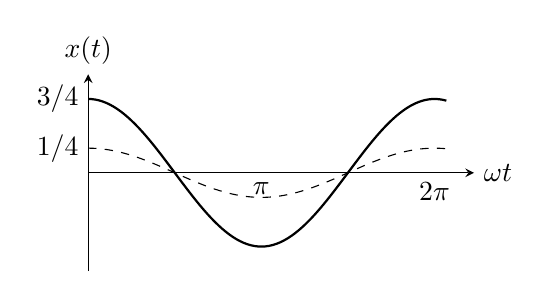
\begin{tikzpicture}[x=.7cm,y=1.25cm,>=stealth]
\draw[->](0,0)--(7,0)node[right]{$\omega t$};\draw[->](0,-1)--(0,1)node[above]{$x(t)$};
\draw[thick,domain=0:6.5,samples=100]plot(\x,{.75*cos(\x r)});
\draw[dashed,domain=0:6.5,samples=100]plot(\x,{.25*cos(\x r)});
\node[left]at(0,.75){$3/4$};\node[left]at(0,.25){$1/4$};\node[below]at(3.14159,0){$\pi$};\node[below]at(6.28318,0){$2\pi$};
\end{tikzpicture}
\end{center}
\step{(2) Densities at the four specified times}
Write $c=\cos\omega t$. For $c\ne0$, the transformation $x=cv$ has inverse $v=x/c$ and absolute Jacobian $1/|c|$. Since $f_V(v)=1$ on $[0,1]$,
\[
f_X(x;t)=\frac1{|c|}\mathbf1_{\{\min(0,c)\le x\le\max(0,c)\}}.
\]
Applying this rule gives
\begin{center}\renewcommand{\arraystretch}{1.6}
\begin{tabular}{c c c}\toprule
Time $t$ & $c=\cos\omega t$ & Density (zero outside the stated interval)\\\midrule
$0$ & $1$ & $1,\quad 0\le x\le1$\\
$\pi/(4\omega)$ & $1/\sqrt2$ & $\sqrt2,\quad 0\le x\le1/\sqrt2$\\
$3\pi/(4\omega)$ & $-1/\sqrt2$ & $\sqrt2,\quad-1/\sqrt2\le x\le0$\\
$\pi/\omega$ & $-1$ & $1,\quad-1\le x\le0$\\\bottomrule
\end{tabular}\end{center}
The negative values of $c$ reverse the support interval; the density coefficient remains positive.
\step{(3) Density at $t_0=\pi/(2\omega)$}
Here $c=0$, so $X(t_0)=0$ for every realization of $V$. The law is a point mass:
\[
\boxed{f_X(x;t_0)=\delta(x),\qquad P\{X(t_0)=0\}=1.}
\]
This is a generalized density; the $1/|c|$ formula cannot be used at $c=0$. The listed nonnegative times implicitly require $\omega>0$.
\newpage
\problem{2.4}{Optional}{61}
A Bernoulli random sequence has independent bits, with $P(B(n)=1)=0.8$ and $P(B(n)=0)=0.2$.
\step{(1) Probability of the word $1011$}
Independence allows the four probabilities to be multiplied:
\begin{align*}
P\{(B(n),B(n+1),B(n+2),B(n+3))=(1,0,1,1)\}
&=0.8\cdot0.2\cdot0.8\cdot0.8\\
&=\boxed{0.1024}.
\end{align*}
\step{(2) Mean word}
Interpret the four-bit word as the random vector
\[
\boldsymbol B=(B(n),B(n+1),B(n+2),B(n+3)).
\]
Each component has mean $\E[B(n)]=0(0.2)+1(0.8)=0.8$. Therefore
\[
\boxed{\E[\boldsymbol B]=(0.8,0.8,0.8,0.8).}
\]
This is the ensemble mean vector, not an actual binary realization.
If instead a word is interpreted as an unsigned binary integer, its expected value is
$\E[8B(n)+4B(n+1)+2B(n+2)+B(n+3)]=15(0.8)=12$.
\step{(3) Most probable word}
A particular word containing $k$ ones has probability
\[
0.8^k0.2^{4-k}.
\]
Replacing a zero by a one multiplies this probability by $0.8/0.2=4>1$. Thus the maximum occurs when all four bits are one:
\[
\boxed{\text{Most probable word: }1111,\qquad P(1111)=0.8^4=0.4096.}
\]
There is no binomial coefficient for a specified word. The factor $\binom4k$ appears only when summing over all words containing $k$ ones.
\newpage
\problem{2.7}{Optional}{61--62}
The process is $X(t)=Vt+X_0$, where $V\sim N(1,1)$ and $X_0\sim N(0,2)$ are independent. In $N(\mu,\sigma^2)$, the second parameter is the variance.
\step{Mean}
At any fixed time $t$, linearity of expectation gives
\[
\boxed{m_X(t)=\E[X(t)]=t\E[V]+\E[X_0]=t.}
\]
\step{Variance}
Independence implies $\Cov(V,X_0)=0$, so
\begin{align*}
\Var[X(t)]&=t^2\Var(V)+\Var(X_0)+2t\Cov(V,X_0)\\
&=t^2+2.
\end{align*}
Thus
\[
\boxed{\sigma_X^2(t)=t^2+2.}
\]
\step{One-dimensional density}
The linear combination of the independent Gaussian variables is Gaussian. One can verify this directly using the characteristic function:
\begin{align*}
\phi_{X(t)}(u)&=\E[\ee^{\jj u(tV+X_0)}]
=\phi_V(tu)\phi_{X_0}(u)\\
&=\exp\left(\jj tu-\frac12t^2u^2\right)\exp(-u^2)\\
&=\exp\left(\jj tu-\frac12(t^2+2)u^2\right).
\end{align*}
This is the characteristic function of $N(t,t^2+2)$. Therefore
\[
\boxed{f_X(x;t)=\frac1{\sqrt{2\pi(t^2+2)}}
\exp\left[-\frac{(x-t)^2}{2(t^2+2)}\right],\qquad x\in\mathbb R.}
\]
As a check, at $t=0$ this reduces to the density of $X_0\sim N(0,2)$.
\newpage
\problem{2.8}{Optional}{62}
For each $n$, $P(I_n=-1)=P(I_n=1)=1/2$, and the Bernoulli sequence has independent samples.
\step{One-dimensional probability density}
The distribution is discrete, so its density is expressed using Dirac impulses:
\[
\boxed{f_{I_n}(x)=\frac12\delta(x+1)+\frac12\delta(x-1).}
\]
Each coefficient is a probability mass. There is no ordinary continuous density.
\step{Mean}
\[
\boxed{m_I(n)=\E[I_n]=(-1)\frac12+(1)\frac12=0.}
\]
Since $I_n^2=1$ for every outcome,
\[
\E[I_n^2]=1,\qquad\Var(I_n)=1.
\]
\step{Covariance function}
By definition,
\[
C_I(n,m)=\E[(I_n-\E I_n)(I_m-\E I_m)]=\E[I_nI_m].
\]
When $n=m$, this equals $\E[I_n^2]=1$. When $n\ne m$, independence gives
\[
\E[I_nI_m]=\E[I_n]\E[I_m]=0.
\]
Consequently,
\[
\boxed{C_I(n,m)=\begin{cases}1,&n=m,\\0,&n\ne m,\end{cases}=\delta_{nm}.}
\]
Here $\delta_{nm}$ is the Kronecker delta for discrete indices. It is distinct from the Dirac delta $\delta(x)$ used in the density. Since the mean is zero, $R_I(n,m)=C_I(n,m)$ as well.
\newpage
\problem{2.11}{Optional}{62}
\begingroup\small
\step{The stated assumption needs care}
The textbook states \emph{pairwise} independence of $A,B,\Theta$. This does not imply independence of $AB$ and $\Theta$. Assume the moments below exist. Pairwise independence does give
$\E[X(t)]=\E[Y(t)]=0$, because each amplitude is independent of the uniform phase.
\step{(1) Cross-correlation under the stated assumptions}
Set $\alpha=\omega t_1$, $\beta=\omega t_2$. The identity
$\sin a\cos b=\tfrac12[\sin(a-b)+\sin(a+b)]$ yields
\[
\boxed{R_{XY}(t_1,t_2)=\tfrac12\E[A]\E[B]\sin(\alpha-\beta)
+\tfrac12\E[AB\sin(\alpha+\beta+2\Theta)].}
\]
The last expectation is not determined by pairwise independence. Thus the stated information does not specify a unique cross-correlation.

For a concrete counterexample, let $Z$ be an independent equiprobable sign, let
$h(\Theta)=\operatorname{sgn}(\sin2\Theta)$, and set $A=Z$, $B=Zh(\Theta)$.
Both $A$ and $B$ are independent of $\Theta$; $A$ and $B$ are also independent since $h$ is an equiprobable sign. Yet $AB=h(\Theta)$, and
\[
R_{XY}(0,0)=\E[h(\Theta)\sin\Theta\cos\Theta]
=\tfrac12\E|\sin2\Theta|=\frac1\pi\ne0.
\]
Values of $h$ at its finitely many zeros do not affect these probabilities.
\step{Common intended answer under the stronger assumption}
If $A,B,\Theta$ are \emph{mutually} independent (or $(A,B)$ is independent of $\Theta$, in addition to $A\perp B$), the phase average of the last term is zero. Then
\[
\boxed{R_{XY}(t_1,t_2)=\tfrac12\E[A]\E[B]\sin\omega(t_1-t_2).}
\]
This extra assumption is needed for this familiar formula; it is not silently inferred from the question.
\step{(2) Orthogonality, uncorrelatedness, and independence}
Since both means are zero, $C_{XY}=R_{XY}$. Hence orthogonality and uncorrelatedness are equivalent here, but cannot be decided from the stated information alone. Under the stronger assumption and $\omega\ne0$, they hold for all pairs of times exactly when $\E[A]\E[B]=0$.
Equal-time orthogonality alone, $R_{XY}(t,t)=0$, is weaker than orthogonality for every pair of times.

Statistical independence does not follow even when $R_{XY}\equiv0$. For example, take mutually independent equiprobable signs $A,B$ and an independent uniform phase. Then $\E A=\E B=0$, but
$X(t)^2+Y(t)^2=1$. More explicitly, each of $|X(t)|>\sqrt3/2$ and $|Y(t)|>\sqrt3/2$ has probability $1/3$, while their intersection is impossible. Thus even the equal-time variables are dependent. Independence is possible in degenerate cases such as $A\equiv0$; the given assumptions do not settle it.
\endgroup
\newpage
\problem{2.18}{Optional}{62}
\step{Mean vector and covariance matrix}
Write $X_0=X(0)$, $X_1=X(1/2)$, $X_2=X(1)$, and set $c=\cos(1/2)$, $s=\sin(1/2)$. Then
\[
\boldsymbol\mu=\begin{bmatrix}2\\2\\2\end{bmatrix},\qquad
\boldsymbol C=8\begin{bmatrix}1&c&\cos1\\c&1&c\\\cos1&c&1\end{bmatrix}.
\]
\step{Why the ordinary three-dimensional density does not exist}
Let $\boldsymbol a=(1,c,\cos1)^{\mathrm T}$ and
$\boldsymbol b=(0,s,\sin1)^{\mathrm T}$. The cosine difference identity gives
\[
\boldsymbol C=8(\boldsymbol a\boldsymbol a^{\mathrm T}+\boldsymbol b\boldsymbol b^{\mathrm T}).
\]
Thus $\operatorname{rank}(\boldsymbol C)\le2$. Its upper-left $2\times2$ determinant is $64s^2>0$, so its rank is exactly $2$, and $\det\boldsymbol C=0$.
The vector $\boldsymbol q=(1,-2c,1)^{\mathrm T}$ satisfies $\boldsymbol C\boldsymbol q=0$. Therefore
\[
\Var\bigl[(X_0-2)-2c(X_1-2)+(X_2-2)\bigr]=0,
\]
so the centered expression is zero almost surely. All probability lies on a plane:
\[
\boxed{(X_0-2)-2c(X_1-2)+(X_2-2)=0.}
\]
Consequently, an ordinary density with respect to three-dimensional volume cannot be written. The nonsingular Gaussian PDF formula is inapplicable.
\step{A valid generalized density}
Put $z_i=x_i-2$. The pair $(X_0,X_1)$ is nonsingular Gaussian with covariance $8\begin{bmatrix}1&c\\c&1\end{bmatrix}$. Combining its density with the plane constraint gives
\[
\boxed{f(x_0,x_1,x_2)=\frac1{16\pi|s|}
\exp\left[-\frac{z_0^2-2cz_0z_1+z_1^2}{16s^2}\right]
\delta(z_2-2cz_1+z_0).}
\]
Integration over $x_2$ removes the delta with unit Jacobian, leaving a normalized bivariate density. Equivalently, a description valid without a PDF is
\[
\boxed{\phi(\boldsymbol u)=\exp\left(\jj\boldsymbol u^{\mathrm T}\boldsymbol\mu-\tfrac12\boldsymbol u^{\mathrm T}\boldsymbol C\boldsymbol u\right).}
\]
The requested ordinary 3D PDF does not exist for the covariance given in the textbook.
\end{document}
